\section{\textbf{Existing Work }}\label{sec:relatedwork}
To place the paper's contribution in context and identify the gap the work is intended to fill, a short literature survey will provide.
We will touch on a brief overview of industrial automation's rival approaches, from Fieldbus to TSN, TSN over 5G in 3GPP Rel.15 and beyond. There were complete solutions and methods to connect field controllers, sensors, and actuators, which Fieldbus technology has granted\cite{thomesse2005fieldbus}. Those make it flexible regarding the architecture and give it the ability to support particular Qos for different applications. Nevertheless, Fieldbus Foundation, a not-for-profit organization, designed standards that increase operability, safety, therefore lowering cost when employing Fieldbus technology. Hence Fieldbus Foundation could guarantee the tested devices to ensure that they meet Fieldbus Foundation specifications and identified with \textsurd FF  for interoperability assurance. Consequently, Fieldbus technology was the ideal solution, and it took over at the A level in industrial automation from 1970 until November 2012, when the TSN Task Force was formed\cite{shoshani2010industrial}.
Time-sensitive networking (TSN) is a collection of standards under development by the IEEE 802.1 \cite{TSN2019_study}.The race was frantic among engineers and researchers working in industrial automation to make wired networks meet the need for time-critical systems. The reason for this was the inefficiency of the original IEEE 802.3 Ethernet standard. Besides, protocols based on Ethernet, like TCP, UDP, and IP, typically do not recognize real-time requirements.
The race was frantic among engineers and researchers working in industrial automation to make wired networks meet the need for time-critical systems. The reason for this was the inefficiency of the original IEEE 802.3 Ethernet standard. Besides, protocols based on Ethernet, like TCP, UDP, and IP, typically do not recognize real-time requirements. Therefore, the Open Systems Interconnection model (OSI model) modification rises to the highest level to match the conditions of the real-time application, which gives a strong impetus to improve the Industrial Ethernet schemes abilities. i.e.,
To overcome obstacles to standard Ethernet and protocol compatibility TCP/IP or UDP/IP with real-time systems requirements\cite{danielis2014survey}. Nevertheless, Ethernet's progress constant over the decades has seen its way into protocols such as Profinet, PowerLink, EtherCAT, and EtherNet/IP \cite{thomesse2005fieldbus}.
  


  \begin{figure}

\centering
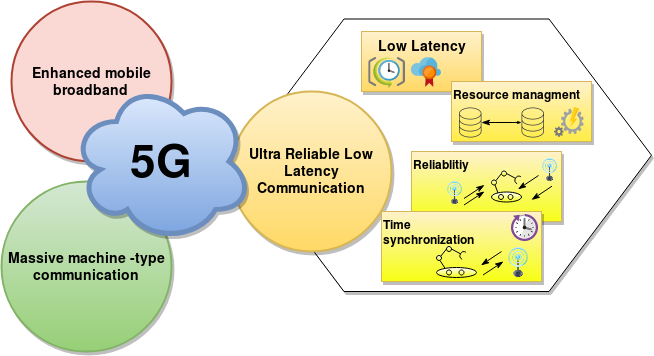
\includegraphics[scale=0.45]{images/5g-tsn-etr-figure01.png}
\caption{5G URLLC overview of TSN components \cite{Ericsson2019}}
\label{fig:5G_URLLC_TSN}
\end{figure}
 
  

\begin{figure}

\centering
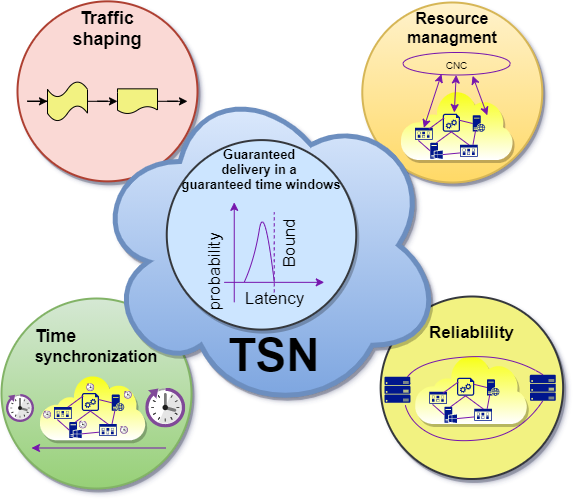
\includegraphics[scale=0.45]{images/TSN toolbox.png}
\caption{Valuable tools within the TSN toolbox that enable deployments in industrial automation \cite{embeddedcomputing2020}.}
\label{fig:TSN_toolbox}
\end{figure}
 

% -------------------------------------------------------------------------------
% The literature survey is a broad and shallow account of the field, which helps
% to place the contribution of the paper in context. It is part of the motivation
% of the paper, because it helps to identify the gap that this work is trying to
% fill, and explain why it is important to fill this gap. Rather than a list of
% disconnected accounts of other people's work, you should try to organise it
% into a story: What are the rival approaches? What are the drawbacks of each?
% How has !the battle between different approaches progressed? What are the major
% outstanding problems? (This is where you come in.)
% -------------------------------------------------------------------------------
\sidenote{intro}
As a review from the above, TSN standards are essentially for IEEE Std 802.3 Ethernet, which indicates they employ all the advantages of standard Ethernet, such as universality, flexibility, and economic operation price.
Various worthy tools are included in those standards like reliability, time synchronization, traffic shaping, resource management, as shown in figure
\textbf{\ref{fig:TSN_toolbox}}
TSN characteristics are developed upon the base IEEE 802.1 bridging standards, making them vital to be carried in industrial automation.


3GPP also provided the conditions for high data rates and traffic densities in 3GPP TS 22.261\cite{5G_Ser_req_nex_gen2018study}; in this 50Mbps is the essential requirement of eMBB service for down link (DL). Up Link (UL) and DL requirement for high data rates and traffic densities can be seen in the \textbf{table}
\textbf{\ref{table:Performance_requirements_highdatarates_traffic_densities}}. 
 



  
%\todoshort{This survey focuses on \ac{WATER} and \ac{Greedy Computing}\ldots\ac{Greedy Computing}}.

%\sidenote{gap 1}
%\todotext{related work 1}



\begin{table}[h!]
\centering
\begin{tabular}{|p{1.8 cm}| p{1.8 cm} |p{1.8 cm}| p{2 cm}| p{2 cm}| p{2 cm}|} 


 \hline
 \cellcolor[HTML]{23a5e2} \color[HTML]{ffffff} \textbf{Scenario} &\cellcolor[HTML]{23a5e2} \color[HTML]{ffffff} \textbf{Experience data rate (DL)}  & \cellcolor[HTML]{23a5e2} \color[HTML]{ffffff} \textbf{Experience data rate (UL)} &\cellcolor[HTML]{23a5e2}\color[HTML]{ffffff} \textbf{Area Traffic Capacity (DL)}   &\cellcolor[HTML]{23a5e2} \color[HTML]{ffffff} \textbf{Area Traffic Capacity (UL)}    & \cellcolor[HTML]{23a5e2}\cellcolor[HTML]{23a5e2} \color[HTML]{ffffff}\textbf{Overall user density }  \\ 
 \hline
 Urban & 50 Mbps &   25 Mbps &  100 \break   Gbps/km2 &     50 \break $Gbps/km^2$  &   $10000/km^2$   \\ 
  \hline
 Rural &     50  Mbps &  25   Mbps &   1 \break   $Gbps/km^2$  &  500 \break  $Gbps/km^2$  & $100/km^2$  \\
  \hline
 Indoor hotspot &    1 Gbps &    500 Mbps &  15  \break   $Tbps/km^2$  &    2 \break $Tbps/km^2$  &   $250000/km^2$  \\
  \hline
 Dense urban &   300 Mbps &  50 Mbps &   750 \break  $Gbps/km^2$  &  125 \break   $Gbps/km^2$  &  $25000/km^2$  \\
  \hline
High- speed vehicle &    50 Mbps &   25 Mbps &    100  \break  $Gbps/km^2$  &   50  \break $Gbps/km^2$  &   $4000/km^2$  \\ [1ex] 
 \hline
\end{tabular}
\caption{Performance requirements for high data rates and traffic densities\cite{5G_Ser_req_nex_gen2018study}.}
\label{table:Performance_requirements_highdatarates_traffic_densities}
\end{table}



\begin{figure}
\centering
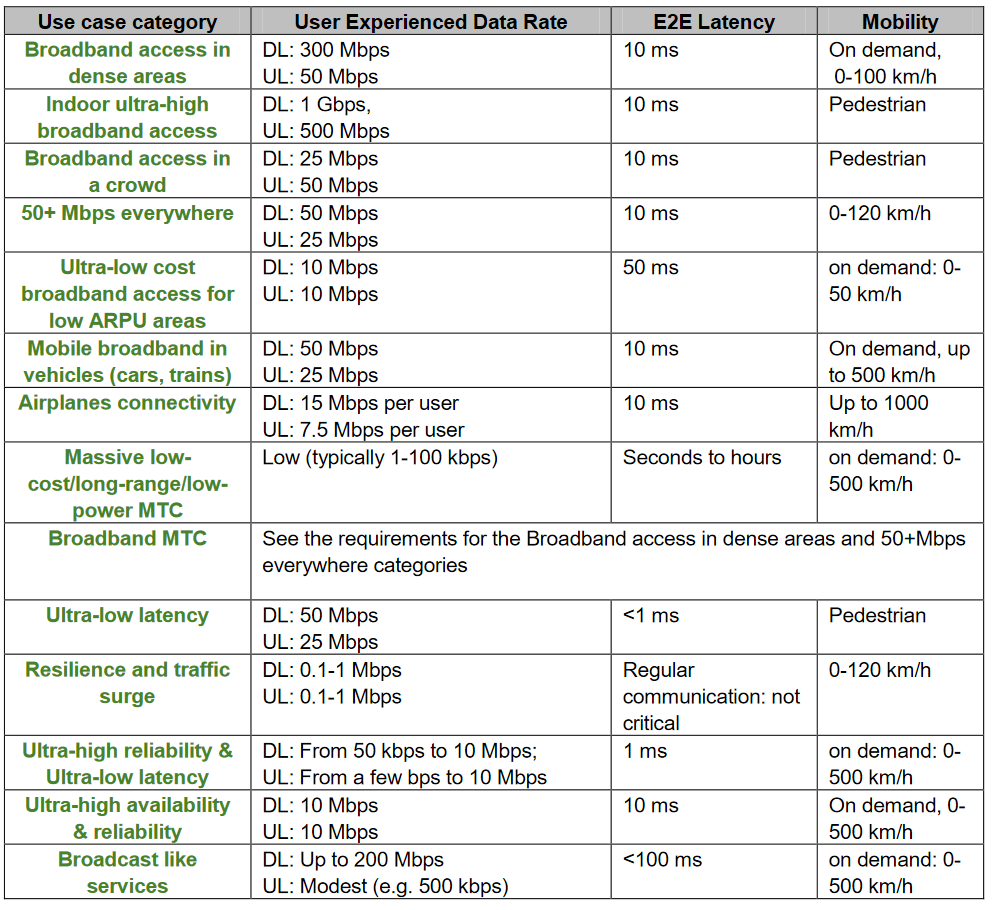
\includegraphics[scale=0.58]{images/User Experience Requirements.png}
\caption{User Experience Requirements\cite{alliance20155g}.}
\label{fig:User_Experience_Requirements}
\end{figure}



\subsection{5G Network Architecture}
3GPP determined the specification of the 5G architecture. 3GPP defined the 5G architecture
in two methods, first as a service-based and the second reference point architecture, which shows the intercommunication between network functions \cite{5G_Tech_Spec_Group_Ser2018study}.
\begin{itemize}
    \item Service-based architecture (SBA) describes the network function (e.g., AMF) of the control plane and also defines how it can authorize other network functions to access the services of other network functions. You can see the SBA in figure \textbf{\ref{fig:5G_SBA}
    \item Reference point architecture explains how the NF services are interacting with the Network function. All of these interactions represented by a point-to-point reference (e.g., N5) between two network functions (e.g., UDM and NRF).  As it shown in figure} \textbf{\ref{fig:5G_Reference_Point_Architecture}}
\end{itemize}


\begin{figure}

\centering
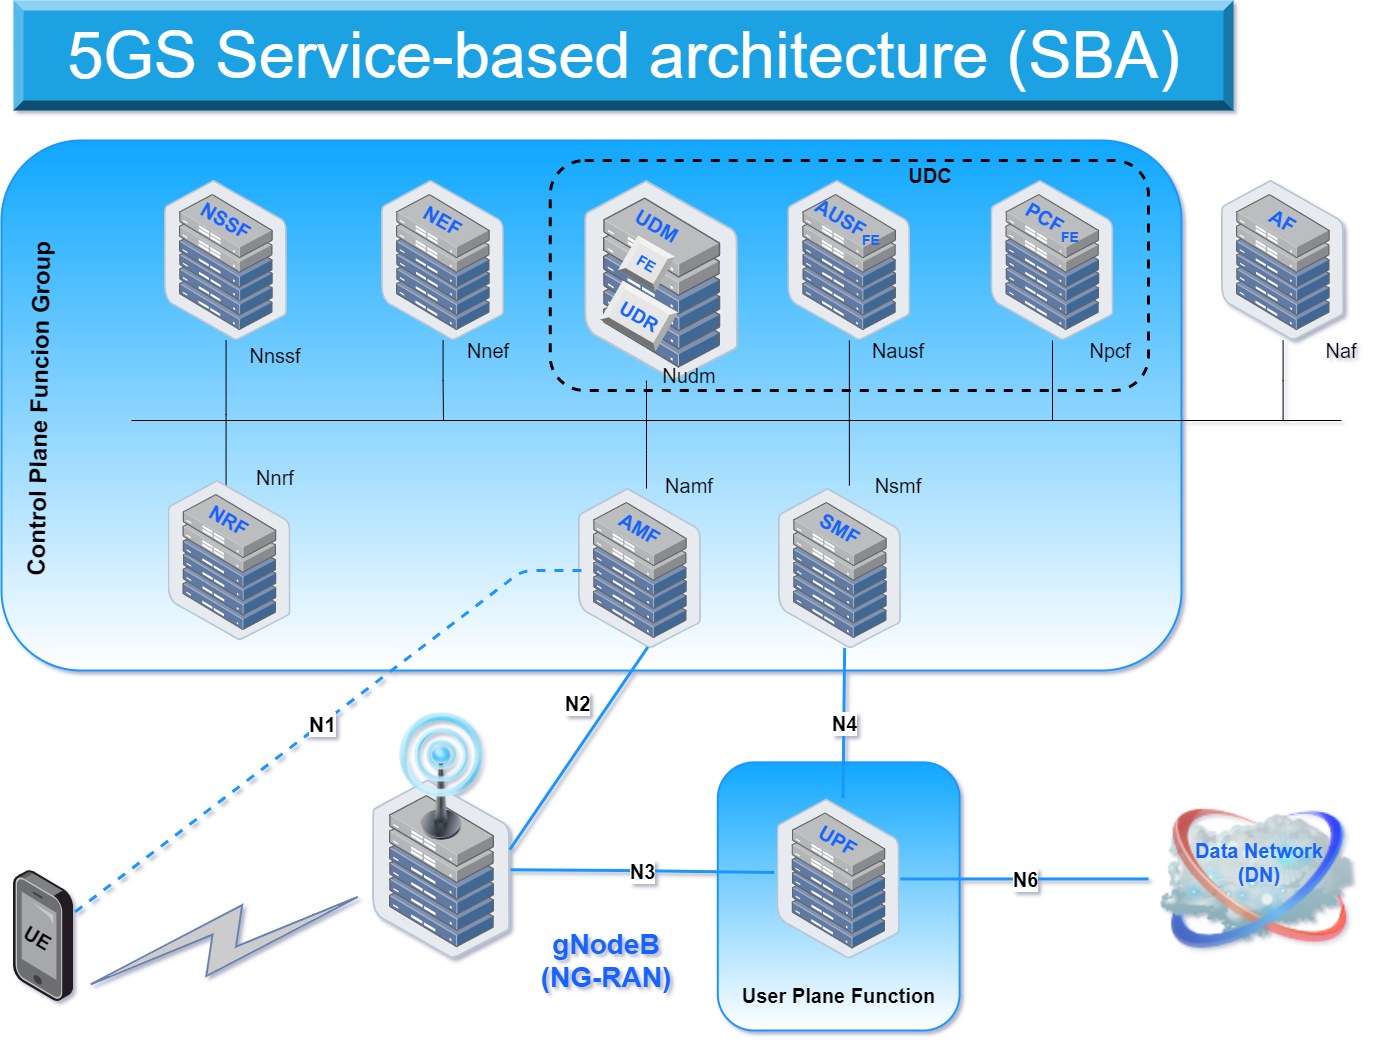
\includegraphics[scale=0.25]{images/5G_SBA.png}
\caption{5GS Service-based architecture (SBA)\cite{5G_Sys_arch_5Gsystem2018study}.}
\label{fig:5G_SBA}
\end{figure}
 
  
\begin{figure}

\centering
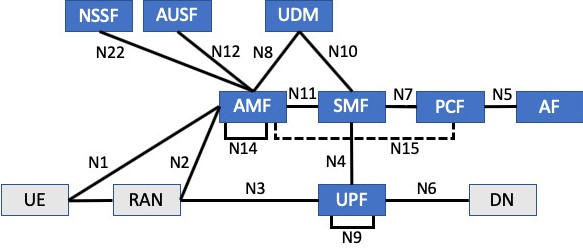
\includegraphics[scale=0.60]{images/5G_Reference_Point_Architecture.png} 
\caption{5G Reference Point Architecture}
\label{fig:5G_Reference_Point_Architecture}
\end{figure}

All essential elements of our research are discussed in the 3GPP release 15 specifications when the 5G service-based architecture (SBA) was reviewed. The fundamental technological components in the 5G core network are the separation of control plane and user plane, service-based interface (SBI), modularization, and network function virtualization. SBA Architecture provides a single API calling interface.  All the network functions (NF) are interconnected via an interface for calling the other NF. 
After Authorization, the network functions (NFs) able to access the other NF using SBI. Network function virtualization (NFV) empowers the network function to be virtualized and deployed on any cloud environment. The support of virtualization in the 5G, the limits between traditional Evolved Packet Core (EPC) network components (MME, SGW, and PGW) will come to exit \cite{5G_Tech_Spec_Group_Ser2018study}.

In 5G Service-Based architecture, Many advantages noticed; independent logical network, sharing the infrastructure either wholly or partly, and being deployed on different infrastructure. I.e., 5GC  Supports network slicing. Furthermore, SBA interfaces are beneficial; 5GC promotes working with 3rd parties and can customize network slice capabilities via AF\cite{5G_Tech_Spec_Group_Ser2018study}.
Another important feature; 5G architecture empowers us to take full advantage of the most advanced virtualization and software technologies. The SBA architecture provides a foreseen performance and flexibility for the network. The following are the 5GC network functions\cite{5G_Sys_arch_5Gsystem2018study}:
\begin{itemize}
    \item AMF: Access and Mobility Management Function - PCF: Policy Control Function.
    \item SMF: Session Management Function - UPF: User Plane Function.
    \item NRF: Network Repository Function - AF: Application Function
    \item NEF: Network Exposure Function - UDM: User Data Management.
    \item AUSF: Authentication Server Function - NSSF: Network Slice Selection Function.
    \item SBI: Service Based Interfaces (Namf, Nsmf, Nudm, Nnrf, Nnssf, Nausf, Nnef, Nsmsf, Nudr, Npcf)
 
\end{itemize}



\textbf{Table}
\textbf{\ref{table: 5G_interfaces_and_the_functional_Description}}  indicates 5G Interfaces and Functional Description of them.
\hfill \break
Another significant technical concept is Network Slicing, clearly “5G slice”, which strengthens the communication service of a particular connection model with a particular method of handling the User-Plane and Control-Plane for this service. To this purpose, a 5G slice is composed of 5G network functions (NF) and precise RAT settings combined together for the exact use case or business model.
figure
\textbf{\ref{fig:Network_Slicing_for_different_use-cases}} represents an instance of multiple 5G slices concurrently served on the same infrastructure\cite{alliance20155g}. 
 
 \begin{table}[h!]
\centering
\begin{tabular}{|p{2.3cm}| p{8.5 cm} |} 

 \hline
 \cellcolor[HTML]{23a5e2} \color[HTML]{ffffff} \textbf{5G interfaces} &\cellcolor[HTML]{23a5e2} \color[HTML]{ffffff} \textbf{Functional Description}    \\ 
 \hline
N1 & Between UE and AMF (Access and Mobility Management Function)  \\ 
  \hline
N2 & Between RAN (Radio Access Network) or gNB (i.e. 5G base station) and AMF  \\ 
  \hline
N3 & Between RAN or gNB (i.e. 5G base station) and UPF (User Plane Function) \\ 
  \hline
N4 & Between SMF (Session Management Function) and UPF
  \\ 
 \hline
  N5 & Between PCF (Policy Control Function) and AF (Application Function).
  \\ 
  \hline
N6 & Between UPF and DN (Data Network)
  \\ 
  \hline
N7 & NG7 is reference point between SMF and PCF 
  \\ 
  \hline
N8 & Between Unified Data Management (UDM) and AMF  \\ 
  \hline
N9 &  Between two core UPFs \\ 
\hline
  N10 &  Reference point between UDM and SMF\\ 
  \hline
N11 & Between SMF and SMF  \\ 
  \hline
N12 & Between AMF and AUSF (Authentication Server Function)    \\ 
  \hline
N13 & Between UDM and AUSF  \\ 
  \hline
N14 & Between two AMFs  \\ 
\hline
  N15 & Between PCF and AMF (in Nonroaming scenario)  \\ 
  \hline
\end{tabular}
\caption{Shows the 5G Interfaces and Functional Description.}
\label{table: 5G_interfaces_and_the_functional_Description}
\end{table}

 
 
 
 
 
 
 
 
 
 
 


\begin{figure}

\centering
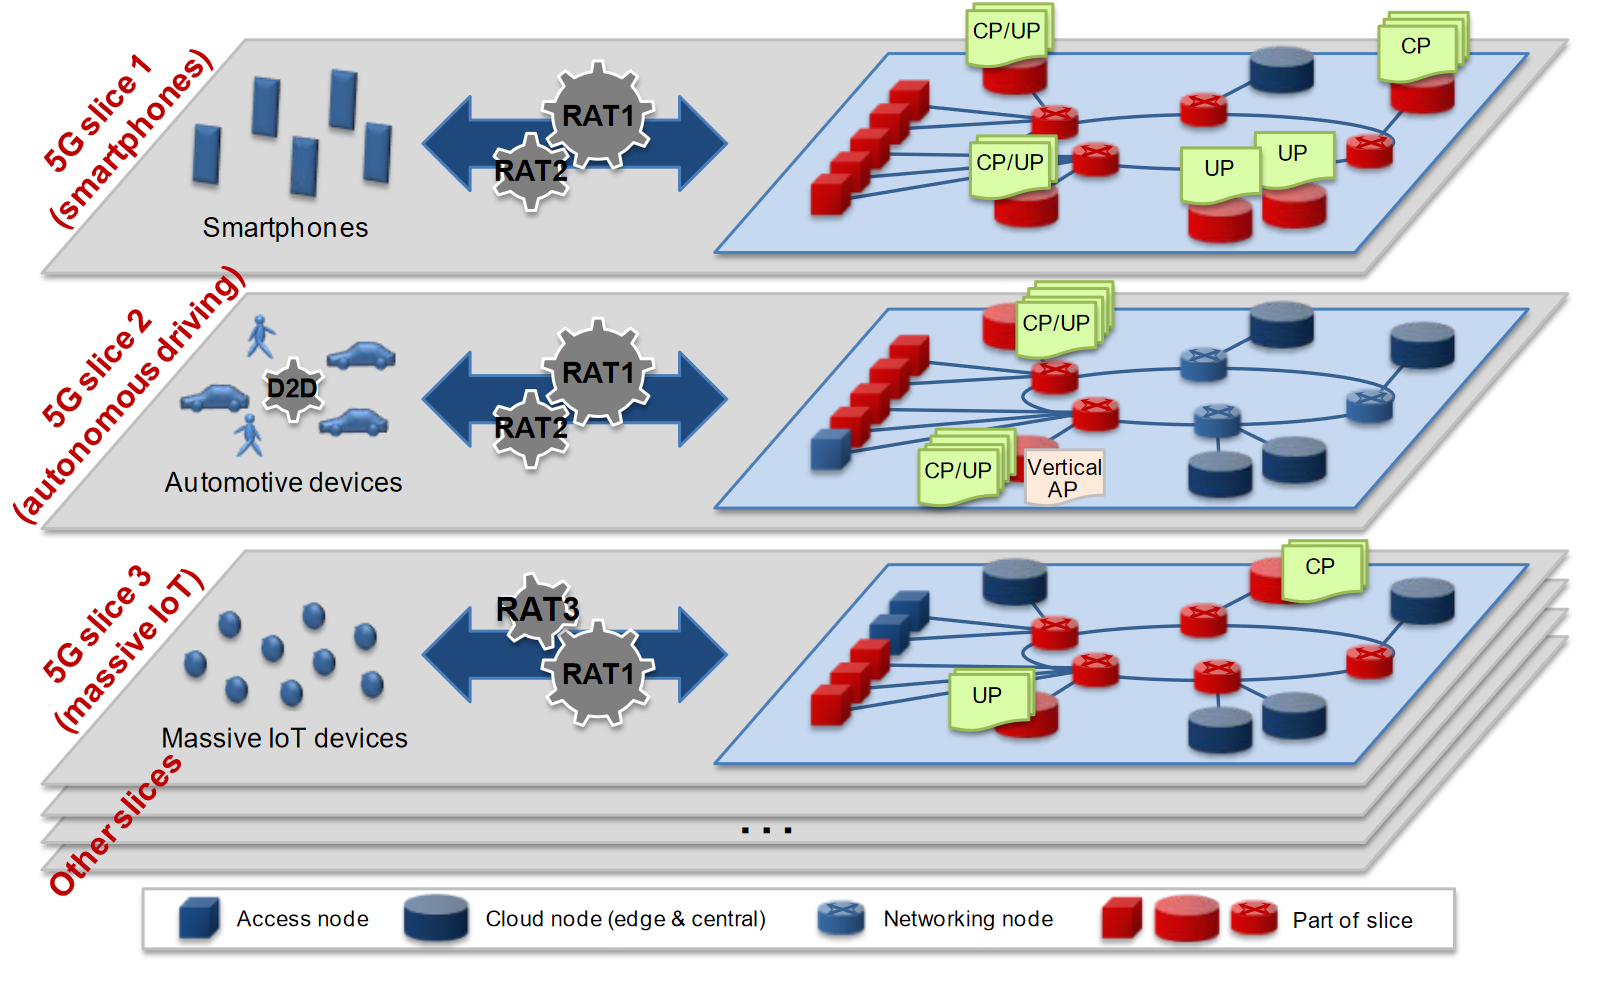
\includegraphics[scale=0.33]{images/Network Slicing for different use-cases.png}
\caption{Network Slicing for different use-cases \cite{alliance20155g}.}
\label{fig:Network_Slicing_for_different_use-cases}
\end{figure}


\subsection{5GC-TSN Integration Scenarios}
The Integration of the 5G core network and TSN has many possibilities. This Thesis will handle three scenarios of them. Every scenario has its unique advantages to award them to particular user applications\cite{5gacia2021_study}. 
 
\begin{itemize}
    \item Scenario 1:
     Within the first scenario, we have the production sectors for the production area. The connection between those isles is using Industrial Ethernet technology \cite{5gacia2021_study}.
Consequently, all communication endpoints give network interfaces according to a similar model. In this scenario, 5GS supports the data interchange amongst the isles, which becomes a demand in Industry 4.0 and digitization \cite{Seijo2019}. 
In this instance, figure
\textbf{\ref{fig:Scenario_1-Connected_homogeneous_islands}}
 shows that 5GC networks are not affected by this scenario, while the focus is restricted to the Radio Access Network (RAN) and the backhaul of the 5GS figure}
\textbf{\ref{fig:The_role_5GS_bridgesindustrial_automation}(A)}.


\begin{figure}

\centering
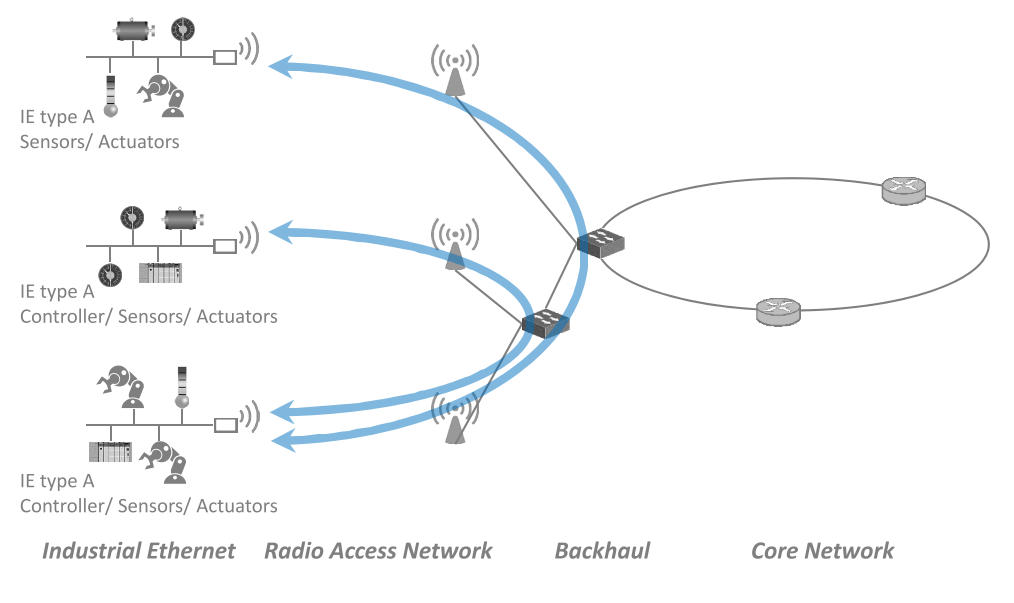
\includegraphics[scale=0.50]{images/Scenario 1- Connected homogeneous islands.png}
\caption{Scenario 1: Connected homogeneous isles \cite{Neumann2018}.}
\label{fig:Scenario_1-Connected_homogeneous_islands}
\end{figure}


\item Scenario 2:
      

This scenario is an ideal decision for utilizing cloud-based control \cite{givehchi2014control}. The motivation of that is working mechanism and structure. I.e., as a main noticed difference between the first and second scenario, the controller's physical object is moved from an allocated machine at the production line to a virtualized entity in the 5G network\cite{5gacia2021_study}. The complete 5GS is covered in this scenario; since the virtualized controller is connected to the core network. In figure \textbf{\ref{fig:Scenario_2_Virtualized_controller}}, we figure out that, Qos is required at a high level because the entire 5G layout is considered in the control loop. The virtualized controller performs a standard Ethernet IP-based connection\cite{5gacia2021_study}. Conversely, two access methods: Industrial Ethernet or native 5G radio, probably are donated by the actuators or sensors at the production line
figure
\textbf{\ref{fig:The_role_5GS_bridgesindustrial_automation}(B)}.

\begin{figure}

\centering
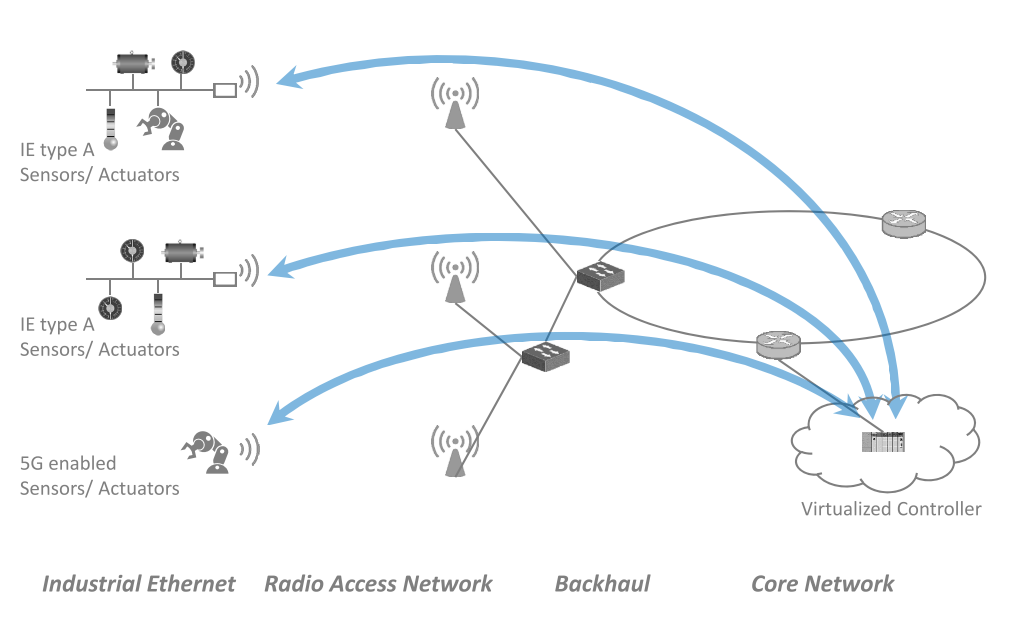
\includegraphics[scale=0.50]{images/Scenario 2- Virtualized controller.png}
\caption{Scenario 2: Virtualized controller \cite{Neumann2018}.}
\label{fig:Scenario_2_Virtualized_controller}
\end{figure}
    
    
    \item Scenario 3:
 A surprise that snatched the spotlight between the three scenarios is scenario 3 shown in figure
\textbf{\ref{fig:The_role_5GS_bridgesindustrial_automation}(C)}. It is similar to the second scenario in terms of a  virtualized controller but is distinct from its design, including a remote production entity connected to 5GC Network \cite{5gacia2021_study}. Hence, its significant advantage demonstrates by supporting various types of communications technologies: 5G radio, standard Ethernet IP-based protocols,  and different Industrial Ethernet protocols.
Scenario 3 diagram illustrated in figure
\textbf{\ref{fig:Scenario_3_Versatility_with_virtualization_&_remote_site}}.



\begin{figure}

\centering
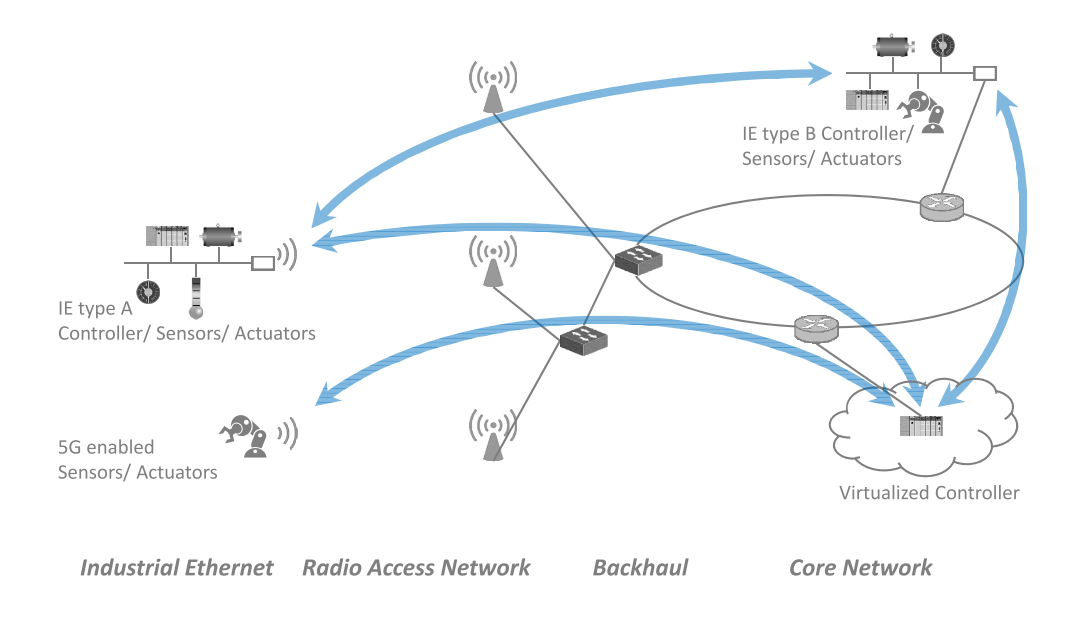
\includegraphics[scale=0.50]{images/Scenario 3- Versatility with virtualization and remote site.png} 
\caption{Scenario 3: Versatility with virtualization and remote site \cite{Neumann2018}.}
\label{fig:Scenario_3_Versatility_with_virtualization_&_remote_site}
\end{figure}


%end scenarios
\end{itemize}
The mentioned scenarios have the feasibility to apply through many use cases of 5GC-TSN integration, which takes its ways in Industrial automation \cite{3gpp2018study}.
Domains that could benefit from the first scenario include;
mobile robots, closed-loop control in process automation, connectivity for the factory floor, mobile control panels, or modular assembly areas. On the other hand, Scenario 2 concerns control-to-control communication, process monitoring, extensive sensor networks,  plant asset management. Last but not least, Scenario 3 is fit for inbound logistics or remote access and maintenance \cite{Neumann2018}.

In addition, Mobility indicates the system’s ability to support continuous service activity for movable users. Furthermore, the identified 5G use cases show that 5G networks will support an increasingly large spectrum of static users/devices to mobile users. 
Regardless of the massive support for 5G networks of a large number of mobile and fixed nodes, 5GS should support mobility-on-demand only. From low mobility or stationary devices like smart meters to very high mobility, like high-speed trains/airplanes \cite{alliance20155g}. In all cases, the conditional speed between the network edge and the user refers to the mobility needs. In other words,  The harmony of the user's activity must be guaranteed.  Use case specific mobility requirements are shown in figure
\textbf{\ref{fig:User_Experience_Requirements}}.




\begin{figure}

\centering
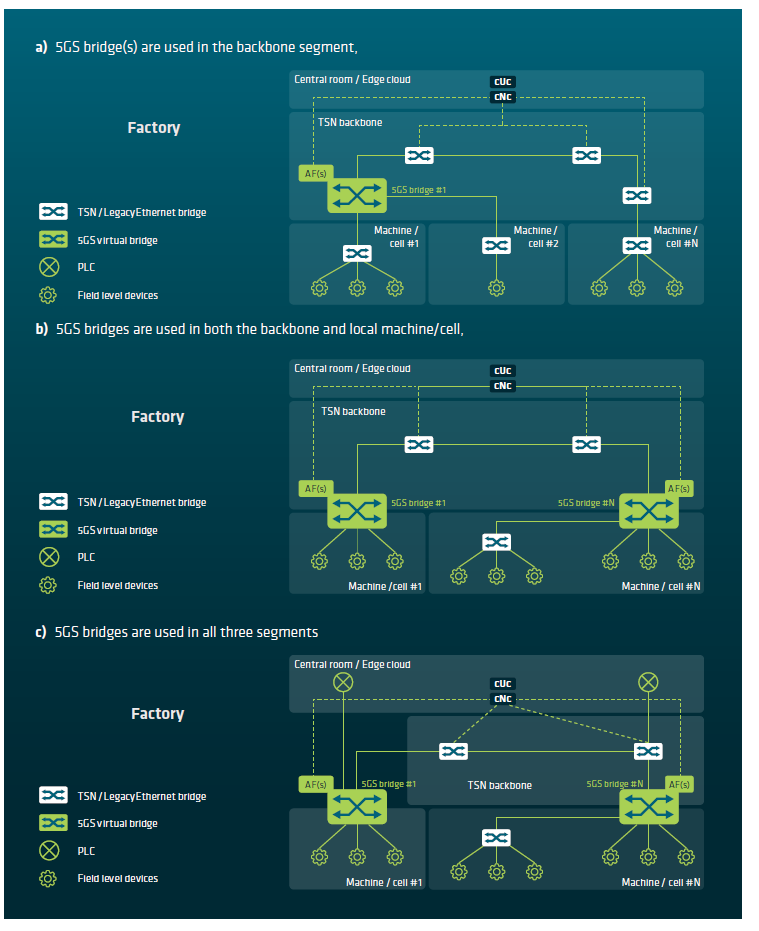
\includegraphics[scale=0.60]{images/The role of 5GS bridges in industrial automation.png} 
\caption{The role of 5GS bridges in industrial automation\cite{5gacia2021_study}.}
\label{fig:The_role_5GS_bridgesindustrial_automation}
\end{figure}

